\documentclass[12pt]{article}
 \usepackage[margin=1in]{geometry} 
\usepackage{amsmath,amsthm,amssymb,amsfonts}
\usepackage{subfigure}
\usepackage{graphicx}

\usepackage{hyperref}
 
\newcommand{\N}{\mathbb{N}}
\newcommand{\Z}{\mathbb{Z}}
\newcommand{\beq}{\begin{equation}}
\newcommand{\eeq}{\begin{equation}}

\setlength{\parindent}{0pt}
\setlength{\parskip}{1em}

\usepackage{color}

 
\begin{document}

 
\title{Notes on 1D plot covariances}
%\author{Author}
\maketitle

The number of objects in pixel $i$ is $N_i$.

In the absence of clustering, $N_i$ is just a poisson sampling so the the covariance matrix is


\begin{equation}
{\bf {\rm Cov}_{w=0}}(N_i,N_j) = \delta_{ij}{\bar N}
\end{equation}

where $\delta_{ij}$ is the Kronecker delta function, and ${\bar N}$ is the average number count per pixel. 

Since $w_{\rm true}(\theta)$ is just the covariance of the overdensity field. When we add clusteirng, the covariance of $N_i$ looks something like this

\begin{equation}
{\bf {\rm Cov}}(N_i,N_j) = \delta_{ij}{\bar N} + {\bar N}^2 w_{\rm true}(\theta_{ij})
\end{equation}

where $\theta_{ij}$ is the separation between pixel $i$ and $j$. I think we are assuming the noise on ${\bar N}$ itself is small in the second term for now. It is a little unclear to me right now what to do when $i=j$ as there will be some beyond poission noise coming from the sample variance of the clustering. Maybe this depends on the size of the pixel? I will come back to this later.....

For the 1d plots we are summing many pixels in an SP bin $k$. We will call this sum $N^{(SP)}$ and we will call the number of pixels in SP bin $k$, $N^{\rm pix}_{k}$.

\begin{equation}
N^{(SP)}_{k} = \sum_{i { \ \rm in \ } k} N_{i}
\end{equation}

In the absence of clustering, the covariance of this would be 

\begin{equation}
{\bf {\rm Cov}_{w=0}}(N^{SP}_k, N^{SP}_l) = \delta_{kl} {\bar N} N^{\rm pix}_{k}
\end{equation}

with clustering it is

\begin{equation}
{\bf {\rm Cov}}(N^{SP}_k, N^{SP}_l) =  {\bf {\rm Cov}}( \sum_{i { \ \rm in \ } k} N_{i}, \sum_{j { \ \rm in \ } l} N_{j})
\end{equation}
\begin{equation}
{\bf {\rm Cov}}(N^{SP}_k, N^{SP}_l) =  \sum_{i { \ \rm in \ } k} \sum_{j { \ \rm in \ } l} {\bf {\rm Cov}}(N_i, N_j) 
\end{equation}
\begin{equation}
{\bf {\rm Cov}}(N^{SP}_k, N^{SP}_l) =  \sum_{i { \ \rm in \ } k} \sum_{j { \ \rm in \ } l} \left[ \delta_{ij}{\bar N} + {\bar N}^2 w_{\rm true}(\theta_{ij}) \right]
\end{equation}
\begin{equation}
{\bf {\rm Cov}}(N^{SP}_k, N^{SP}_l) =  \delta_{kl} {\bar N} N^{\rm pix}_{k} + \sum_{\theta} N^{\rm (pix \ pairs)}_{kl}(\theta) {\bar N}^2 w_{\rm true}(\theta) + {(i=j \ \rm term?)}
\end{equation}

where $N_{\rm pix \ pairs}(\theta)$ is the number of pairs of pixels separated by $\theta$ which can be obtained from treecorr or other pair counting codes. Assuming your $w(\theta)$ and pair counts are in discrete bins.

If there is an actual systematic signal, I think we could just use the real number counts as the poisson term

\begin{equation}
{\bf {\rm Cov}}(N^{SP}_k, N^{SP}_l) =  \delta_{kl} N^{SP}_{k} + \sum_{\theta} N^{\rm (pix \ pairs)}_{kl}(\theta) {\bar N}^2 w_{\rm true}(\theta) + {(i=j \ \rm term?)}
\end{equation}

\section{Example on DES Y6 log-normal mocks}

I have taken 100 Lognormal mocks designed to match the Y6 maglim sample and computed the covariance of the 1d airmass correlation from the mocks. I then compare this to the above calculation using the same $w(\theta)$ used to generate the mocks. 

\begin{figure}[h]
    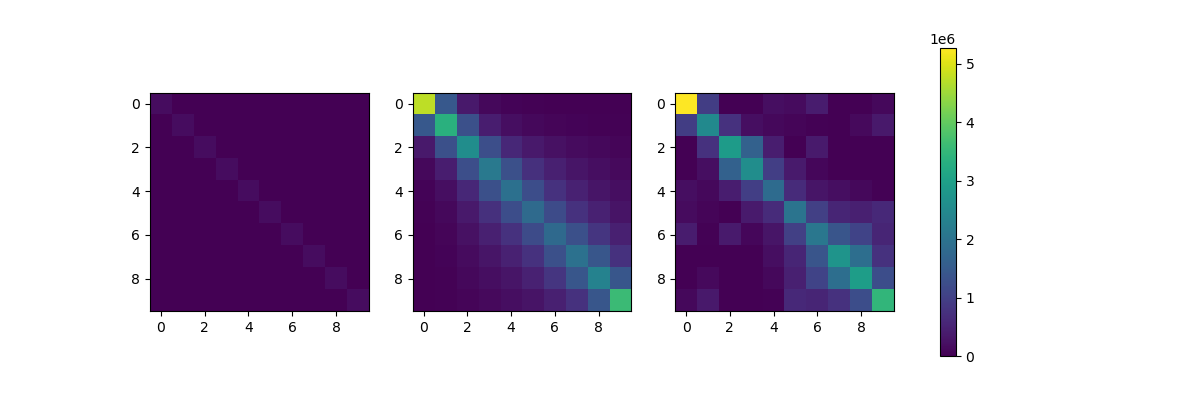
\includegraphics[width=1.2\linewidth]{../test/cov_eq.png}
    \caption{}
    \label{fig:example}
\end{figure}

\begin{figure}[h]
    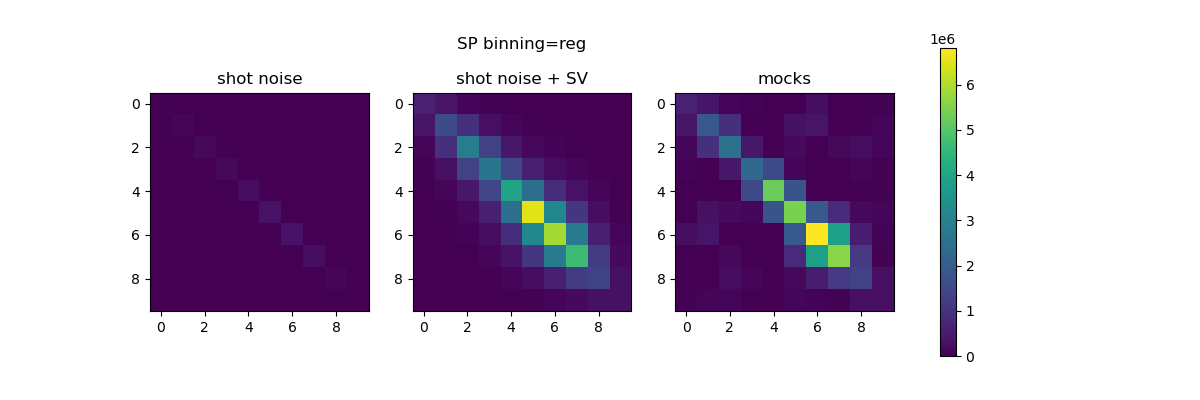
\includegraphics[width=1.2\linewidth]{../test/cov_reg.png}
    \caption{}
    \label{fig:example}
\end{figure}

\begin{figure}[h]
    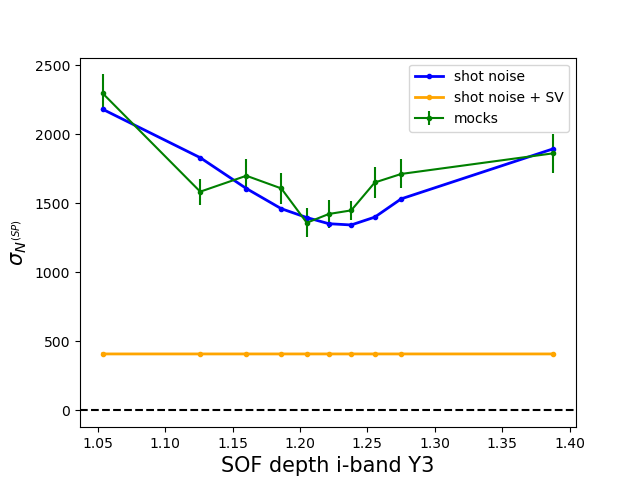
\includegraphics[width=0.75\linewidth]{../test/diagonal_eq.png}
    \caption{}
    \label{fig:example}
\end{figure}

\begin{figure}[h]
    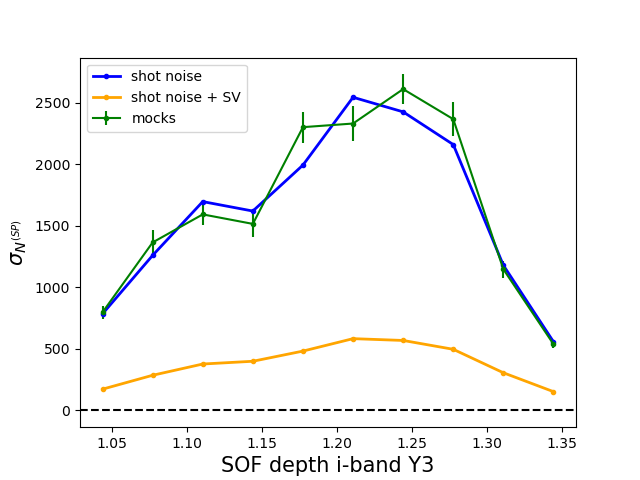
\includegraphics[width=0.75\linewidth]{../test/diagonal_reg.png}
    \caption{}
    \label{fig:example}
\end{figure}


\section{Things to check}

Does the $i=j$ term matter? I'm guessing it will matter more for large pixels 

What are the requirements  wtheta binning, and max/min separation

Can this be extended to multiple maps simultaniously? e.g could we make a data vector that contains the correlations with many SP maps, fit them simultaniously and use this method to compute the large covariance matrix (e.g. 10 SP maps, 10 bins per map, we make a 100x100 covariance)





\end{document}




